\chapter{Interpretation of Morphogen Gradients by a Bistable Circuit}
\label{chapter:double-exclusive}
\begin{music}
    \parindent10mm \instrumentnumber{1} \setstaffs1{1} 
    \generalmeter{\meterfrac34} \generalsignature{0}
    \startextract
		\Notes\zq d\qu a \qu f\qu h\enotes\bar
        \Notes\zq h\qu b\hl i\enotes
    \zendextract
\end{music}
\epigraph{\textit{the clear water's surface reflects
growth}}{Serenade of Water --- Ocarina of Time}\section{Preface}

This chapter contains a published article which resulted from an interdisciplinary collaboration in synthetic cell biology with Station B at Microsoft Research Cambridge. The aim of Station B was to improve all phases of the \emph{design--build--test--learn} workflow (Figure \ref{fig:dbtl}). While specific questions in developmental biology were addressed in the publication, the research was conducted with the wider purpose of identifying bottlenecks in synthetic biology workflow and designing software and automation tools to alleviate those bottlenecks. In particular, the workflow should enable the optimisation of experimental conditions that would yield specific design goals within biomanufacturing pipelines. Applications could range from increasing the yield on \emph{leghemoglobin} through the genetic manipulation of synthetic yeast in the production of plant-based meats, to optimisation of transfection protocols for the production of cell-based therapies, through to engineering bacteria or algae for bio-compatible dye production and application.

\subsection{Problem Statement \& Context}

The aim of this project is to reconstitute and control minimal self-organisation mechanisms which are believed play crucial roles in developmental biology. To this
end \textit{E. Coli} has been genetically engineered to produce orthogonal responses to two different input signals --- henceforth this organism will be referred to as the \textit{double exclusive reporter} circuit \cite{Grant2016OrthogonalBehavior}. The colony of reporters serve as a reduced model for a multi-cellular organism during embryonic stages of development. While patterns with sharp boundaries have successfully been realised, producing Turing instabilities remains challenging as the system needs to be such that patterns develop before the colony reaches stationary phase. The role of theory and computation in this project is to help identify the parameter regimes that produce controllable and self-organised patterns.

\subsection{Contributions}

\textbf{Grisha Szep} is co-second author with \textbf{Om Patange} (University of Cambridge, UK). \textbf{Paul Grant}, \textbf{Neil Dalchau}, \textbf{Jacob Halatek} and \textbf{Andrew Phillips} (all Microsoft Research Cambridge, UK) conceived and designed the study. \textbf{Paul Grant} designed and built the genetic circuits. \textbf{Paul Grant}, \textbf{Om Patange} and \textbf{Valerie Coppard} (Microsoft Research Cambridge, UK) performed the experiments. \textbf{Grisha Szep}, \textbf{Jacob Halatek} and \textbf{Neil Dalchau} conceived and implemented theory and modelling and wrote the supplementary information. All authors analysed and interpreted the data. \textbf{Paul Grant} and \textbf{Andrew Philips} wrote the main text. All authors provided input into the manuscript. The contributions of \textbf{Grisha Szep} the main text (Sections \ref{double-exclusive:abstract}--\ref{afterword:inference}) and supplementary (Appendix \ref{appendix:double-exclusive}), labelled as they appear in the \emph{Nature Communications 11} include:
\begin{itemize}
    \item \textbf{Figure 1.b} Spatial simulations of parameterised model
    \item \textbf{Figure 2.a-b} Calculation of region of bistability predicted by the parameterised model using arc-length continuation algorithms
    \item \textbf{Figure 3.b-e} Wrote bespoke inference code for quantification of boundary velocity from microscopy movies and comparison to theoretical model
    \item \textbf{Figure 4.d-e} Spatial simulations of the parameterised model. Novel state-space analysis of boundary formation and bistability
    \item \textbf{Figure S10.c} Spatial simulations analysed in state-space
    \item \textbf{Figure S13} A novel method for quantifying hysteresis in the flow cytometry experiments as population separation
    \item \textbf{Figure S25-S26} Bistability analysis of parameterised models and comparison to qualifications from flow cytometry
    \item \textbf{Figure S27-S33} Simulations of boundary velocity, novel way of understanding them in state space and bespoke inference methods for quantification of boundary velocity from microscopy movies
    \item \textbf{Figure S36} State space geometry for model with feedback loops
    \item \textbf{Supplementary Sections 2.2-2.4} Wrote sections outlining the methods for extracting bistability regions from data and models with and without feedback loops
    \item \textbf{Movies 1-5} Simulations of expression boundary formation
    \item \textbf{Code} Released code with documentation in the GitHub Repository \href{https://github.com/gszep/double-exclusive-reporter}{\texttt{github.com/gszep/double-exclusive-reporter}}
\end{itemize}

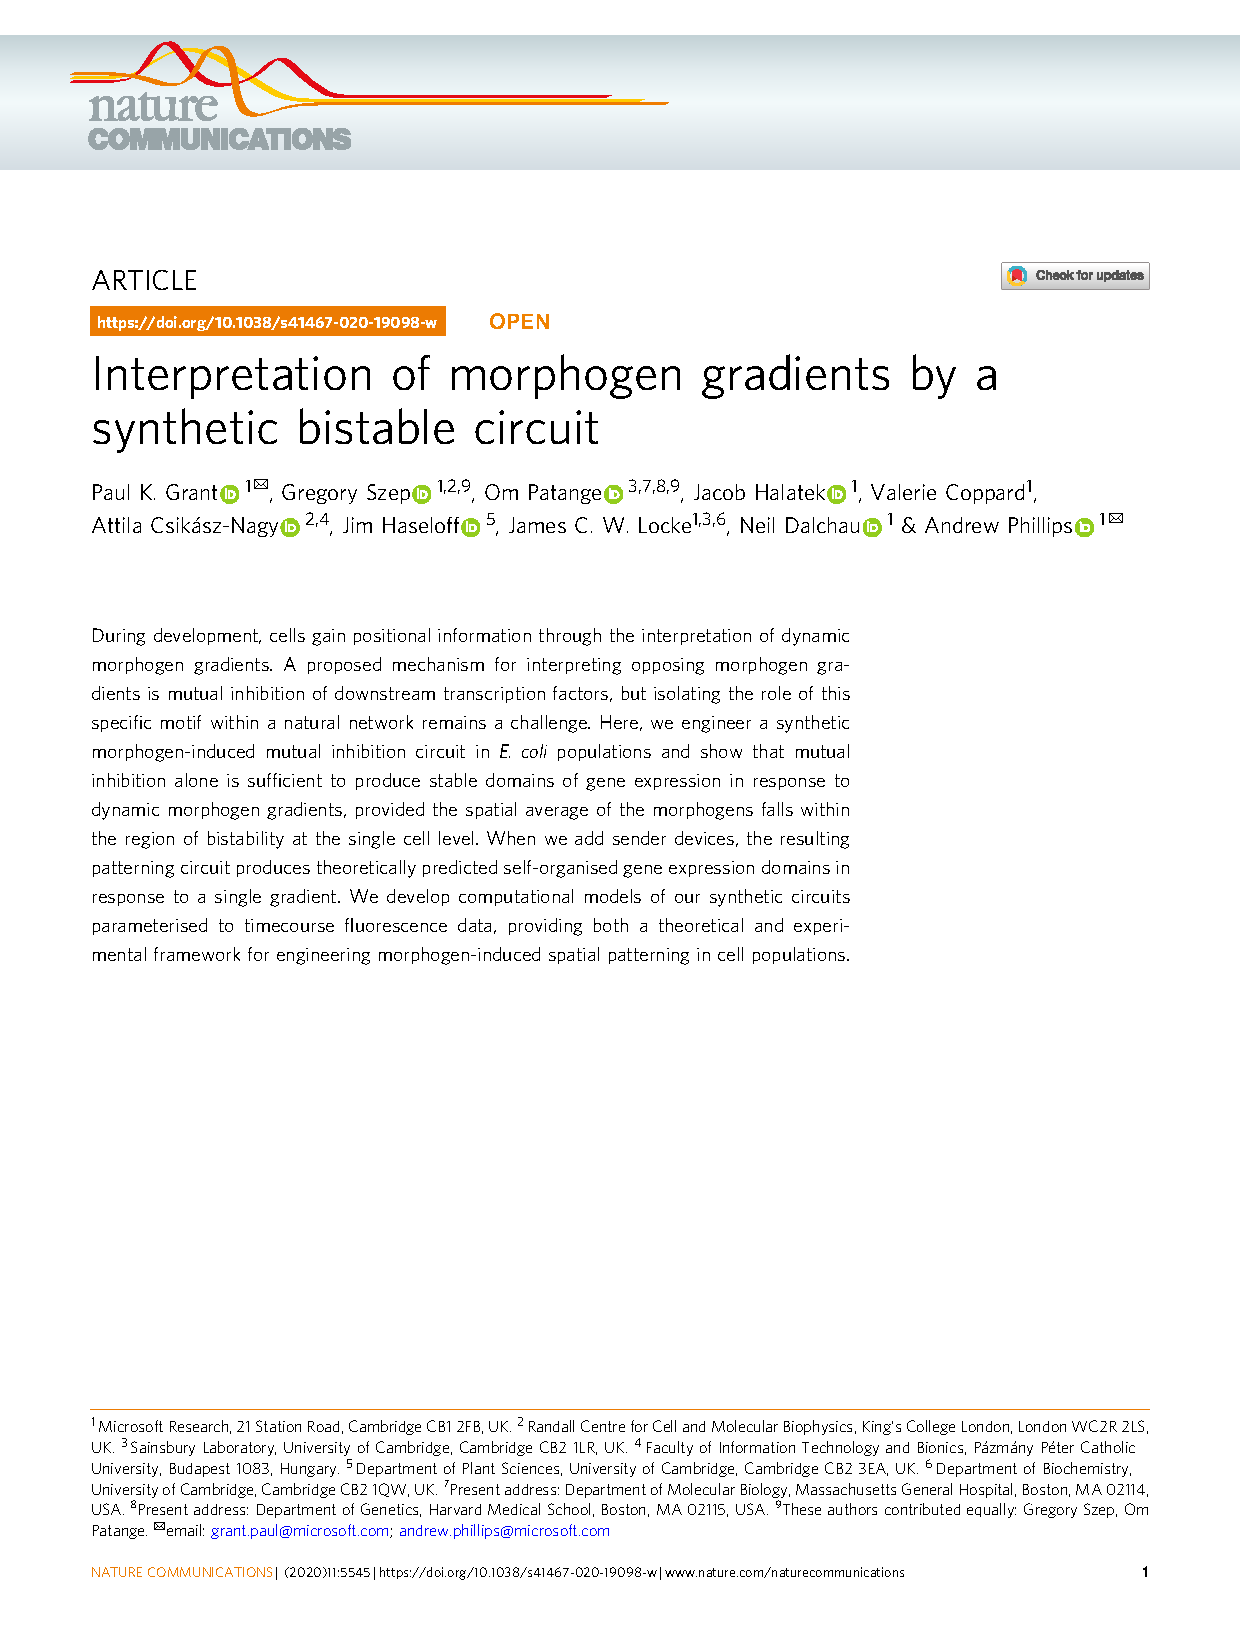
\includepdf[pages=1-8, offset=75 -90, scale=0.85, frame,
        clip,trim=10mm 5mm 10mm 0mm,
        pagecommand={}, addtotoc={
        1,section,1,Abstract,double-exclusive:abstract,
        2,section,1,Introduction,double-exclusive:introduction,
        2,section,1,Results,double-exclusive:results,
        2,subsection,2,Engineering mutual exclusivity,double-exclusive:exclusivity,
        3,subsection,2,Mutual inhibition results in bistability,double-exclusive:bistability,
        4,subsection,2,Hysteresis produces stable boundaries,double-exclusive:boundaries,
        4,subsection,2,A secondary gradient creates self-organised domains,double-exclusive:self-organisation,
        5,section,1,Discussion,double-exclusive:discussion,
        6,section,1,Methods,double-exclusive:methods,
        6,subsection,2,Plasmid construction,double-exclusive:plasmids,
        6,subsection,2,Plate fluorometer assay,double-exclusive:plates,
        6,subsection,2,Flow-cytometric analysis of hysteresis,double-exclusive:flow,
        7,subsection,2,Microfluidics,double-exclusive:microfluidics,
        7,subsection,2,Microfluidics microscopy,double-exclusive:microscopy,
        7,subsection,2,Solid culture assays,double-exclusive:cultures},
    addtolist={
        2, figure, {\textit{Fig. 1}\quad A synthetic gene circuit for morphogen interpretation.}, fig:double-exclusive:overview,
        3, figure, {\textit{Fig. 2}\quad Mutual inhibition produces bistability.}, fig:double-exclusive:bistability,
        5, figure, {\textit{Fig. 3}\quad Formation of stable boundaries.}, fig:double-exclusive:boundaries,
        6, figure, {\textit{Fig. 4}\quad Addition of a Relay circuit creates self-organised domains of gene expression.}, fig:double-exclusive:relay
}]{publications/double-exclusive.pdf}

\section{Afterword}
\label{afterword:inference}
During the early days of this collaboration a lot of effort went into estimating differential equation parameters $\theta$ from time-course fluorescence microplate measurements using a hierarchical Monte Carlo approach (details in Appendix \ref{appendix:double-exclusive:inference}). In this approach, the parameters of isolated sub-modules and growth dynamics are estimated first and then propagated them as priors for the estimation of the more complex model \cite{Dalchau2019ScalableCircuits}. This enables the iterative refinement of both the \emph{in silico} model and the synthetic \emph{E. coli} as new data is collected without having to infer parameters from scratch at each step. As the study progressed, more data on the synthetic system was collected to precisely sample the bistable and switching behaviour in the form of single cell trajectories (Figure \ref{fig:double-exclusive:bistability}c) and flow cytometry (Figure \ref{fig:double-exclusive:flow-hysteresis}). This data type was not compatible with the inference approach we had built and therefore the best we would do was qualitatively compare the data to the results of parameter continuation \cite{Veltz2020BifurcationKit.jl} on the \emph{in silico} models (Figure \ref{fig:double-exclusive:bistability}a--b and Figures \ref{fig:double-exclusive:degradation-models}--\ref{fig:double-exclusive:growth-rate-sensitivity}).

One of the problems with microplate data is that it is not possible to detect multi-modality in fluorescence distributions that could indicate a population of mixed phenotypes. By inferring single cell model parameters from population level data, we are relying on the structure of the model to restore the information on the single cell level. We do not need to do this, however, if only we inferred parameters from the multi-modality that can be directly observed in single cell trajectories and flow cytometry data. Furthermore, we have to consider that our design goals, the cusp bifurcation, lives in state-space rather than the time-domain. This suggests that we should process our data (perhaps using the approach described in Figure \ref{fig:cusp-sampling}) to extract bifurcations. Using bifurcation data prioritises qualitative dynamics over any attempt at inferring kinetic parameters \cite{Stumpf2019ParameterBifurcations}.
\clearpage
The disconnect between the data domain used for parameter inference and the domain of the design goals motivated investigating \emph{inverse bifurcation analysis} methods. Such methods try and find parameter regimes that lead to desired cusp and limit points directly. However, searching for bifurcating parameter regimes within a model is a difficult task, and few methods exist in the literature. We found some contributions where bespoke methods were applied to specific model structures, but would not generalise to arbitrary models \cite{Otero-Muras2018Optimization-basedModels,Otero-Muras2014ACurves}. Other approaches were based on sampling parameter sets naively and checking for the existence of a bifurcation \cite{Lu2006InverseSystems,Chickarmane2005BifurcationTool}. But, there was no end-to-end differentiable method that took advantage of bifurcation theory directly. We therefore attempted to fill this gap in the literature by developing a methodology based on differentiable continuation in Chapter \ref{chapter:inference}. In doing so, we have elucidated the importance of fitting qualitative before quantitative features within datasets.